\documentclass[10pt,a4paper,oneside]{scrartcl}
\usepackage[latin1]{inputenc}
\usepackage{amsmath}
\usepackage{amsfonts}
\usepackage{amssymb}
\usepackage{makeidx}
\usepackage{graphicx}
\usepackage{booktabs}
\usepackage{tikz}
\usepackage[
	   style=ieee
	   ]
	   {biblatex}
\usepackage{mathtools}
\author{}
\title{Trie}
\date{}
\addbibresource{~/modules/References.bib}
\begin{document}
\maketitle
\paragraph{Notation}: \texttt{trie}
\paragraph{Description}: A structure for organizing sequential data hierarchically. Members of a previous generation can spawn infinitely many members of the next generation, but the data cannot be read out of sequence. In other words a parent can spawn any number of children, but cannot skip a generation. This ensures that all the data in a trie are related to each other properly. 

A simple kind of trie that everyone has used is a list: \\

\centering
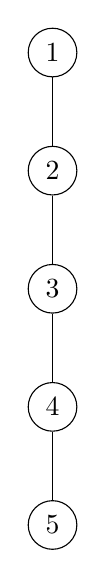
\begin{tikzpicture}[sibling distance=10em,
  every node/.style = {shape=circle,
    draw, align=center,
    top color=white, bottom color=blue!0}]]
  \node {1}
      child { node {2}
	child { node {3}
	  child { node {4}
	    child { node {5} } } } };
\end{tikzpicture}

\printbibliography
\end{document}

